\documentclass[10pt]{exam}

\usepackage{amssymb, amsmath, amsthm, mathrsfs, multicol, graphicx}
\usepackage{tikz}

 \def\d{\displaystyle}
\def\?{\reflectbox{?}}
\def\b#1{\mathbf{#1}}
\def\f#1{\mathfrak #1}
\def\c#1{\mathcal #1}
\def\s#1{\mathscr #1}
\def\r#1{\mathrm{#1}}
\def\N{\mathbb N}
\def\Z{\mathbb Z}
\def\Q{\mathbb Q}
\def\R{\mathbb R}
\def\C{\mathbb C}
\def\F{\mathbb F}
\def\A{\mathbb A}
\def\X{\mathbb X}
\def\E{\mathbb E}
\def\O{\mathbb O}
\def\U{\mathcal U}
\def\pow{\mathcal P}
\def\inv{^{-1}}
\def\nrml{\triangleleft}
\def\st{:}
\def\~{\widetilde}
\def\rem{\mathcal R}
\def\sigalg{$\sigma$-algebra }
\def\Gal{\mbox{Gal}}
\def\iff{\leftrightarrow}
\def\Iff{\Leftrightarrow}
\def\land{\wedge}
\def\And{\bigwedge}
\def\AAnd{\d\bigwedge\mkern-18mu\bigwedge}
\def\Vee{\bigvee}
\def\VVee{\d\Vee\mkern-18mu\Vee}
\def\imp{\rightarrow}
\def\Imp{\Rightarrow}
\def\Fi{\Leftarrow}

%\def\={\equiv}
\def\var{\mbox{var}}
\def\mod{\mbox{Mod}}
\def\Th{\mbox{Th}}
\def\sat{\mbox{Sat}}
\def\con{\mbox{Con}}
\def\bmodels{=\joinrel\mathrel|}
\def\iffmodels{\bmodels\models}
\def\dbland{\bigwedge \!\!\bigwedge}
\def\dom{\mbox{dom}}
\def\rng{\mbox{range}}
\DeclareMathOperator{\wgt}{wgt}


\def\bar{\overline}


\newcommand{\vtx}[2]{node[fill,circle,inner sep=0pt, minimum size=4pt,label=#1:#2]{}}
\newcommand{\va}[1]{\vtx{above}{#1}}
\newcommand{\vb}[1]{\vtx{below}{#1}}
\newcommand{\vr}[1]{\vtx{right}{#1}}
\newcommand{\vl}[1]{\vtx{left}{#1}}
\renewcommand{\v}{\vtx{above}{}}

\def\circleA{(-.5,0) circle (1)}
\def\circleAlabel{(-1.5,.6) node[above]{$A$}}
\def\circleB{(.5,0) circle (1)}
\def\circleBlabel{(1.5,.6) node[above]{$B$}}
\def\circleC{(0,-1) circle (1)}
\def\circleClabel{(.5,-2) node[right]{$C$}}
\def\twosetbox{(-2,-1.4) rectangle (2,1.4)}
\def\threesetbox{(-2.5,-2.4) rectangle (2.5,1.4)}
\newcommand{\twoline}[2]{\begin{pmatrix}#1 \\ #2 \end{pmatrix}}


\def\circleA{(-.5,0) circle (1)}
\def\circleAlabel{(-1.5,.6) node[above]{$A$}}
\def\circleB{(.5,0) circle (1)}
\def\circleBlabel{(1.5,.6) node[above]{$B$}}
\def\circleC{(0,-1) circle (1)}
\def\circleClabel{(.5,-2) node[right]{$C$}}
\def\twosetbox{(-2,-1.5) rectangle (2,1.5)}
\def\threesetbox{(-2,-2.5) rectangle (2,1.5)}

%\pointname{pts}
\pointsinmargin
\marginpointname{pts}
\bonuspointname{pts}
\marginbonuspointname{pts}
\addpoints
\pagestyle{head}
\printanswers

\firstpageheader{Math 228}{\bf Homework 10\\Solutions}{Due: Wednesday, November 15}


\begin{document}
% \noindent \textbf{Instructions}: Same rules as usual -- turn in your work on separate sheets of paper.  You must justify all your answers for full credit.  Do not consult the Internet.

\begin{questions}
  \question[9] A convex polyhedron is a 3 dimensional geometric figure made up of faces, each of which is a polygon.  Thus a polyhedron has a number of faces, edges and vertices, just like a planar graph.  In fact, you can represent every convex polyhedron as a planar graph.  (``Convex'' means that the interior angle between any two faces is less then $180^\circ$.)
  \begin{parts}
  \part An {\em octahedron} is a regular polyhedron made up of 8 equilateral triangles (it sort of looks like two square-based pyramids with their bases glued together).  Draw a planar graph representation of an octahedron.  How many vertices, edges and faces does an octahedron (and your graph) have?  It might be helpful to decide on these numbers before drawing the graph.
  \begin{solution}
  Since there are 8 triangles, there must be 8 faces.  We can count the number of edges by taking $8 \cdot 3 = 24$, but this is double counting since each edge corresponds to two faces.  Thus there are 12 edges.  We can use Euler's formula to find that there are 6 vertices (and this shows that each vertex is the joining of 4 triangles).

  The planar representation of the graph is:



  \begin{center}
  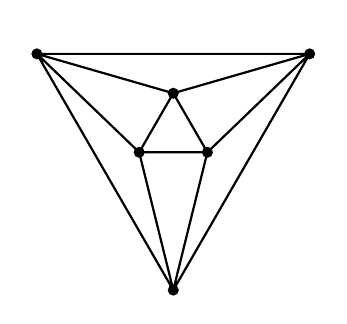
\begin{tikzpicture}
  \coordinate (a) at (30:2);
  \coordinate (b) at (150:2);
  \coordinate (c) at (270:2);
  \coordinate (d) at (90:.5);
  \coordinate (e) at (210:.5);
  \coordinate (f) at (-30:.5);
  \draw[thick] (a) \v -- (b) \v -- (c) \v -- (a) -- (d)\v --(e)\v -- (f)\v --(d) -- (b) -- (e) -- (c) -- (f) -- (a);

  \end{tikzpicture}
  \end{center}


  \end{solution}
  \part The traditional design of a soccer ball is in fact a (spherical projection of a) truncated icosahedron.  This consists of 12 regular pentagons and 20 regular hexagons.  No two pentagons are adjacent (so the edges of each pentagon are shared only by hexagons).  How many vertices, edges, and faces does a truncated icosahedron have?  Explain how you arrived at your answers.  Bonus: draw the planar graph representation of the truncated icosahedron.
  \begin{solution}
  Well, right off we know that the truncated icosahedron has $12+20=32$ faces by counting the number of pentagons and hexagons. Now, because we know that every connected planar graph with $v$ vertices, $e$ edges and $f$ faces satisfied $v - e + f = 2$, we only really need to find out the number of edges or the number of vertices since $v-e=-30$. So, let's maybe try to figure out the number of edges we have. If we think about the number of total edges when the pentagons and hexagons are not attached, we know that we have $5\times 12+6\times 20=180$. But each of these edges is shared with another edge, which means that we have cut the number of edges in half. So, we have $90$ edges, which then gives us $60$ vertices.
  \end{solution}
  \part Your ``friend'' claims that he has constructed a convex polyhedron out of 2 triangles, 2 squares, 6 pentagons and 5 octagons.  Prove that your friend is lying.  Hint: each vertex of a convex polyhedron must border at least three faces.
  \begin{solution}
  So, let's assume for a contradiction that your friend really has constructed a convex polyhedron. Then, we would know that the polyhedron has $15$ faces, $(2\times 3+2\times 4+6\times 5+5\times 8)/2 = 42$ edges, and $v=2+42-15=29$ vertices. Now, using the hint, we also know that the degree of each vertex is at least 3, and the number of edges is half the sum of the degrees.  Thus we have $3v\leq 2e$ but $3\cdot 29$ is not in fact less than $2 \cdot 42$. So we have a contradiction, and your friend is lying.
  \end{solution}
  \end{parts}

  \question[6] Prove that the {\em Petersen graph} (below) is not planar.  Hint: what is the length of the shortest cycle?

  \begin{center}
    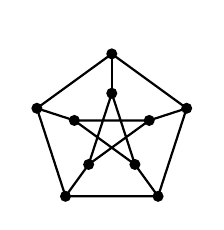
\begin{tikzpicture}[scale=.5]
      \draw[thick] (18:2) -- (90:2) -- (162:2)  -- (234:2) -- (306:2) -- cycle;
      \draw[thick] (18:1) --  (162:1)  -- (306:1) -- (90:1) -- (234:1) --cycle;
      \foreach \x in {18, 90, 162, 234, 306}
      \draw[thick] (\x:1) \v -- (\x:2) \v;
    \end{tikzpicture}
  \end{center}

  \begin{solution}
    \begin{proof}
      Suppose, for contradiction, that the Petersen graph were planar.  Then it would satisfy Euler's formula: $v - e + f = 2$.  Since the graph has 10 vertices and 15 edges, this says that there must be $7$ faces.

      Now let $b$ be the total number of boundaries around all faces when the graph is drawn in a planar way.  Since each edge is used in two boundaries we have $b = 2e$.  On the other hand, each face is surrounded by {\em at least} 5 boundaries, since the shortest cycle (circuit) in the graph contains 5 edges.  Thus $f \le \frac{b}{5}$.  Putting these two facts together we get
      \[f \le \frac{2e}{5}\]
      This is a contradiction, since $7 \not\le \frac{2\cdot 30}{5}$.  Alternatively, the above relationship says that $f \le 6$, but we said $f = 7$ above.

      Therefore the Petersen graph is not planar.
    \end{proof}

  \end{solution}


  \question[9] A {\em tree} is a connected graph with no cycles.
  \begin{parts}
  \part Draw a bunch of trees.  Conjecture a relationship between a the number of vertices and edges in any tree. (For instance, can you have a tree with 5 vertices and 7 edges?)
  \begin{solution}
  After drawing a few trees, you should notice that there is always exactly one more vertices than edges. That is $v=e+1$
  \end{solution}
  \part Explain why every tree with at least 3 vertices has at least one vertex with degree 1 (such a vertex is called a \emph{leaf}.  Hint: try a proof by contradiction.
  \begin{solution}
  Assume for a contradiction that every tree with at least 3 vertices does not have a leaf. Namely, that there are no vertices of degree 1. Then, every vertex must have a degree of 2 or more, but this would imply that we have a cycle! Why? Think about taking a path from one vertex to another. Choose the first vertex and a route to leave it (remember it should have at least two ways to leave). Once I leave that vertex I reach another vertex which also has at least one more way to leave. Keep doing this. Eventually you will get back to one of the vertices that you have already visited and therefore you will have completed a cycle.
  \end{solution}
  \part Prove your conjecture from part (a) by \underline{induction} on the number of vertices. Hint: For the inductive step, you will assume that your conjecture is true for all trees with $k$ vertices, and show it is also true for an arbitrary tree with $k+1$ vertices.  So start with an arbitrary tree with $k+1$ vertices.  Consider what happens when you cut off a leaf and then let it regrow.
  \begin{solution}
  Recall that we need two parts for an induction proof: a base case and an inductive case.
  \begin{proof}
  Let $P(n)$ be the statement ``a tree $T_n$ with $n$ vertices has $n-1$ edges.''
  Base Case: Draw a tree with three vertices. Clearly you have only 2 edges (otherwise you would have a cycle).\\
  Inductive Case: Assume $P(k)$ is true for some arbitrary $3<k<n$.\\
  NTS: $P(k+1)$ is true. That is $T_{k+1}$ has $k$ edges.\\
  Let $T_{k+1}$ be a tree graph with $k+1$ vertices. By part (b) we know that every tree with at least 3 vertices has a leaf, so cut that one leaf off of $T_{k+1}$. Then our tree graph has only $k$ vertices, and by our inductive case has $k-1$ edges. Well, if we let that leaf regrow we will add both one edge and one vertex, which means that we will have a tree graph with $k+1$ vertices and $k-1+1=k$ edges. TBTPOMI we have shown that $P(n)$ is true.
  \end{proof}
  \end{solution}
  \end{parts}



 \question[6] The two problems below can be solved using graph coloring.  For each problem, represent the situation with a graph, say whether you should be coloring vertices or edges and why, and use the coloring to solve the problem.
 \begin{parts}
   \part Your Quidditch league has 5 teams.  You will play a tournament next week in which every team will play every other team once.  Each team can play at most one match each day, but there is plenty of time in the day for multiple matches.  What is the fewest number of days over which the tournament can take place?

   \begin{solution}
     The graph to represent this question is $K_5$, since each vertex (team) is adjacent to (plays) each other vertex (team).  The edges are thus the games that are played.  We cannot have a team play more than one game per day, so we color the edges observing the rule that two edges incident to the same vertex must be colored differently.  Edges that are colored the same \emph{can} be played on the same day, so we are looking for the smallest number of colors needed to color the edges in this way.  You obviously need at least 4 colors, but this does not work.  In fact, there is a coloring using 5 colors, so you need 5 days for the tournament.
   \end{solution}
   \part Ten members of Math Club are driving to a math conference in a neighboring state.  However, some of these students have dated in the past, and things are still a little awkward.  Each student lists which other students they refuse to share a car with; these conflicts are recored in the table below.  What is the fewest number of cars the club needs to make the trip?  Do not worry about running out of seats, just avoid the conflicts.

   \begin{tabular}{l|*{10}{c}}
     Student: & A & B & C & D & E & F & G & H & I & J \\ \hline
     Conflicts: &BEJ&ADG&HJ&BF&AI&DJ&B&CI&EHJ&ACFI
   \end{tabular}
   \begin{solution}
     Here we color the vertices.  The chromatic number of this graph is 3, so three cars are needed.
   \end{solution}
 \end{parts}



\end{questions}
\end{document}
